
\documentclass[
				twoside,
				11pt, a4paper,
				footinclude=true,
				headinclude=true,
				cleardoublepage=empty
]{scrbook}

\usepackage[utf8]{inputenc}
\usepackage{lipsum}
\usepackage[linedheaders,parts,pdfspacing]{classicthesis}
\usepackage{amsmath}
\usepackage{amsthm}
\usepackage{acronym}
\usepackage{algorithm}
\usepackage{algpseudocode}
\usepackage{tikz}
\usetikzlibrary{shapes}
\usetikzlibrary{positioning,arrows}
\usetikzlibrary{decorations.pathreplacing} 

\newtheorem{theorem}{Theorem}[section]


\author{João Valença}
\title{Visualisation and Analysis of Geographic Information: Algorithms and Data Structures}

\begin{document}
\maketitle	

\setcounter{tocdepth}{2} % <-- 2 includes up to subsections in the ToC
\setcounter{secnumdepth}{3} % <-- 3 numbers up to subsubsections
\tableofcontents 

\setcounter{page}{0}
\pagenumbering{roman}

\section*{\huge Abstract}

In recent years, Geographic Information Systems (GIS) have witnessed a large increase in data availability. There is a need to process a large amount of data before it can be managed and analysed. This project aims to develop a GIS application operating through a Web platform in order to allow for a low cost and simplified integration, management and manipulation of georeferenced information. Special emphasis is given to the implementation of efficient clustering algorithms for finding a representative set of points in a map. The approaches covered in this thesis include exact algorithms for solving the \emph{k-centre} problem, as well as approximation algorithms and heuristic methods to solve the \emph{geometric disk cover} problem.

\subsection*{\large Keywords}

Geographic Clustering, Coverage, Geometric Algorithms, k-Centre, Geometric Disk Cover, Real-Time Applications

\section*{\huge Resumo}

Nos últimos anos, os Sistemas de Informação Geográfica (GIS) têm assistido a um grande aumento na quantidade de dados disponíveis. De facto, existe uma necessidade de encontrar uma maneira eficiente de processar grandes quantidades de dados para que tanta informação possa ser facilmente gerida e analisada. Este projeto visa desenvolver uma aplicação GIS para uma plataforma Web, de modo a obter uma integração simples e de baixo custo que manipule e analise dados georeferenciados. Uma ênfase especial é dada à implementação de algoritmos para encontrar um conjunto representativo de pontos num mapa. As abordagens descritas nesta tese incluem algoritmos exactos para resolver o problema do \emph{k-centre}, bem como algoritmos de aproximação e métodos heurísticos para resolver o problema de \emph{geometric disk cover}.

\subsection*{Palavras-chave}

Clustering Geográfico, Cobertura, Algoritmos Geométricos, k-Centre, Geometric Disk Cover, Aplicações de Tempo Real


\cleardoublepage
\chapter{Introduction}
\label{chap:intro}
\lhead{Chapter \ref{chap:intro}. \emph{\nameref{chap:intro}}} % This is for the header

In recent years, there has been a large increase in the amount and availability of geographic data. This new surge of such large quantities of data has prompted a similar rise on the number of applications to capture, store, manipulate and analyse this data.
A lot of these applications share the need to visualise the geographic information in such a way that it can be easily understood by a human.
This is usually done by displaying points of interest on a map so that their relative position or direction can be easily interpreted by the user.

One obstacle when representing large amounts of geographic data is that the sheer number of points to display can be overwhelming for a human, as well as computationally intensive to render for a machine. As such, there is a need to develop and implement a viable way to reliably calculate and display a subset of geographic points, whilst keeping a degree of representativeness of the larger set, so that as little information as possible is absent when the representative subset is shown.

The purpose of this project is to research and develop a real-time algorithm that can analyse geographic data provided by a geographic information system (GIS) infrastructure developed and maintained at Smartgeo. More precisely, the developed algorithm will have to be able to aggregate and select geographic points according to a given a set of criteria. Figure \ref{fig:rep} shows an example of a representative subset of an original, larger set, as well as one possibility for a representative set.

\begin{figure}[H]
	\centering
	\begin{minipage}{0.4\linewidth}
		\centering
		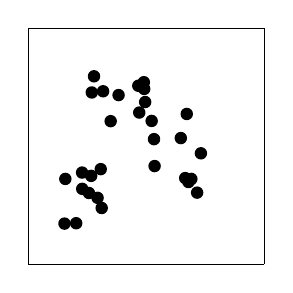
\begin{tikzpicture}[scale=1.5]
			\draw (0,0) -- (2,0);
			\draw (2,0) -- (2,2);
			\draw (2,2) -- (0,2);
			\draw (0,2) -- (0,0);
			
			\fill (0.456,0.778)circle (1.5pt);
			\fill (0.622,0.478)circle (1.5pt);
			\fill (0.457,0.64)circle (1.5pt);
			\fill (0.614,0.807)circle (1.5pt);
			\fill (0.314,0.724)circle (1.5pt);
			\fill (0.533,0.75)circle (1.5pt);
			\fill (0.514,0.605)circle (1.5pt);
			\fill (0.307,0.346)circle (1.5pt);
			\fill (0.406,0.349)circle (1.5pt);
			\fill (0.587,0.564)circle (1.5pt);
			
			\fill (1.065,1.061)circle (1.5pt);
			\fill (1.045,1.215)circle (1.5pt);
			\fill (1.292,1.07)circle (1.5pt);
			\fill (1.381,0.724)circle (1.5pt);
			\fill (1.43,0.608)circle (1.5pt);
			\fill (1.342,1.274)circle (1.5pt);
			\fill (1.329,0.731)circle (1.5pt);
			\fill (1.462,0.941)circle (1.5pt);
			\fill (1.357,0.698)circle (1.5pt);
			\fill (1.07,0.833)circle (1.5pt);
			
			\fill (0.765,1.434)circle (1.5pt);
			\fill (0.557,1.593)circle (1.5pt);
			\fill (0.698,1.213)circle (1.5pt);
			\fill (0.634,1.466)circle (1.5pt);
			\fill (0.979,1.543)circle (1.5pt);
			\fill (0.99,1.375)circle (1.5pt);
			\fill (0.538,1.456)circle (1.5pt);
			\fill (0.932,1.513)circle (1.5pt);
			\fill (0.982,1.486)circle (1.5pt);
			\fill (0.94,1.286)circle (1.5pt);
		\end{tikzpicture}
		\caption*{\footnotesize Original Set}
		\label{fig:badrep}
	\end{minipage}
	\begin{minipage}{0.4\linewidth}
		\centering
		\begin{tikzpicture}[scale=1.5]
		\draw (0,0) -- (2,0);
		\draw (2,0) -- (2,2);
		\draw (2,2) -- (0,2);
		\draw (0,2) -- (0,0);
		
		\fill (0.622,0.478)circle (1.5pt);
		\fill (1.462,0.941)circle (1.5pt);
		\fill (0.765,1.434)circle (1.5pt);
		\end{tikzpicture}		
		\caption*{\footnotesize Representative Set}
		\label{fig:goodrep}
	\end{minipage}
	\label{fig:rep}
\end{figure}

This thesis aims to research, develop, and analyse different algorithms to choose a representative subset of geographic points, whilst being able to dynamically change that set of points via zooming or panning over a geographic region containing a large amount of geographical data. In case the optimal solution algorithms prove to be too slow, heuristic approaches will be implemented. Heuristic algorithms will have their solution quality and speed benchmarked against implicit enumeration algorithms.
The algorithm that is2 deemed the most suitable to solve the task will be integrated in a web framework via the \emph{geojson} and \emph{WFS} (web feature service) geographic data communication standards. Figure \ref{fig:arch} shows the basic concept of the architecture for the web application.

\begin{figure}[!h]
	\begin{center}
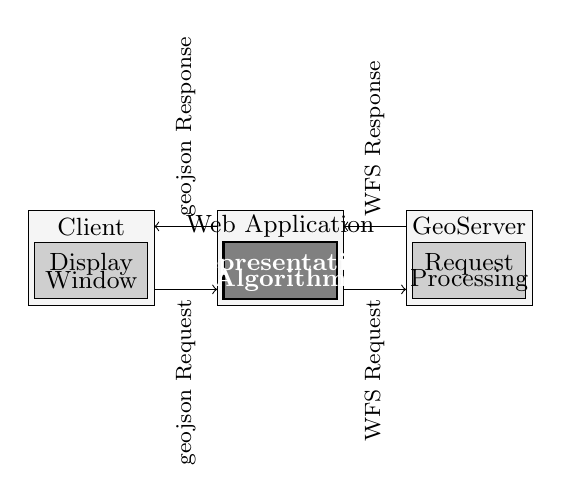
\begin{tikzpicture}[scale=0.4]
	\begin{scope}[]
		\fill[lightgray!15,draw=black] (0,0) rectangle (4,3);
		\fill[lightgray!75,draw=black] (0.2,0.2) rectangle (3.8,2);
		\node at (2,2.5) {\small Client};
		\node at (2,1.3) {\small Display};
		\node at (2,0.8) {\small Window};
	\end{scope}
	\begin{scope}[shift={(6,0)}]
		\fill[lightgray!15,draw=black] (0,0) rectangle (4,3);
		\fill[black!50,draw=black,thick] (0.2,0.2) rectangle (3.8,2);
		\node at (2,2.5) {\small Web Application};
		\node[text=white] at (2,1.3) {\small \textbf{Representation}};
		\node[text=white] at (2,0.8) {\small \textbf{Algorithm}};
	\end{scope}
	\begin{scope}[shift={(12,0)}]
		\fill[lightgray!15,draw=black] (0,0) rectangle (4,3);
		\fill[lightgray!75,draw=black] (0.2,0.2) rectangle (3.8,2);
		\node at (2,1.3) {\small Request};
		\node at (2,0.8) {\small Processing};
		\node at (2,2.5) {\small GeoServer};
	\end{scope}
	
	\begin{scope}[shift={(6,-0.5)},rotate=90]
		\draw[->] (1,2) -- node[left,rotate=90] {\footnotesize geojson Request} (1,0) ;
		\draw[<-] (3,2) -- node[right,rotate=90] {\footnotesize geojson Response} (3,0);
	\end{scope}


	\begin{scope}[shift={(12,-0.5)},rotate=90]
		\draw[->] (1,2) -- node[left,rotate=90] {\footnotesize WFS Request} (1,0) ;
		\draw[<-] (3,2) -- node[right,rotate=90] {\footnotesize WFS Response} (3,0);
	\end{scope}
\end{tikzpicture}
\end{center}
\label{fig:arch}
\end{figure}

The application is meant to function as an independent module capable of being decoupled and used for different clients and/or servers, should the need arise in the future.

Some famous web applications and services perform similar operations that already select from large sets of points. Most of these rely on having different preprocessed layers of information, which contain similarly ranked points. For example, a map of a continent would only request the layer containing the capitals of the visible countries, whilst a map of a singular country would only request the layer containing the cities within the viewing window's coordinates.

This solution requires that a lot of preprocessed data be stored in a fairly large and robust database. It also skips the representation problem by having points with different importance ranks. If any geographic query returns too many points for the application to render, then it could choose to only display the higher ranked ones or, alternatively, repeat the same query to the layer above to reduce the stress. Since this problem requires that no storage space is used, other solutions must be found.

Another approach is done by projecting all points to a limited resolution image format. Mapping vectorial points into a bitmap format with no aliasing means that all points that are closer together than a pixel will likely be rounded off to the same spot, effectively merging the two points.

Explicitly creating an image file may result in a larger file, which may cause problems in a bandwidth-dependant web application. The solution to this would be to round the coordinates of every point to a grid, and only relay the coordinates of the grid that would contain any points. This method, however, would mean a loss of precision increasing with the size of the grid. Furthermore, the points selected would be grid-aligned, and not necessarily correspond with any of the original, vectorial set. This would make for a visual pattern, which would be obvious for a human user. This solution is therefore also not suitable for our purpose.

Since no suitable algorithms were found, new ones had to be designed to properly solve the problem. The first approach interpreted the representation problem as an optimization problem known as \emph{Minimum Coverage Subset}. This problem requires that a number of points is chosen out of the original set to become the representative set. It finds the best possible combination of the original set such points to represent it, with the cardinality constrained to an input value. This constrain meant that the number of representative points must be known before the algorithm is executed, which is not always the case. Because of this particular limitation, and coupled with performance issues, a second approach was made. In this new approach, the algorithm is given a minimum distance between points in the representative set. The algorithm must then find the smallest collection of circles with this distance as their radius such that no point in the set is uncovered. This is known as a \emph{Geometric Disk Cover} problem, and our specific formulation has one extra constraint that makes it so that the circles need to have their centres on points of the original set. Because of the performance issues met in the first approach, this problem was solved using an approximation algorithm, which compromises the quality of the result (within a controlled threshold) in order to be performed in a more reasonable time. 

This report is organized as follows:
Chapter \ref{chap:theory} - \nameref{chap:theory} defines the base theoretical concepts, such as a notion of representativeness, as well as some useful structures used in the algorithms. Chapter \ref{chap:algos} - \nameref{chap:algos} describes the implicit enumeration algorithms implemented for the minimum coverage set problem, as well as an analysis on their time and space complexities. Chapter \ref{chap:approx} - \nameref{chap:approx} describes the approximation algorithm for the geometric disk coverage problem, as well as heuristic accelerations and a space and time complexity analysis. The chapter ends with a proposed solution to the issue of panning the viewing window.
\input{cstudy}
\chapter{Optimal Minimum Coverage Algorithms}
\label{chap:algos}
\lhead{Chapter \ref{chap:algos}. \emph{Deterministic Algorithms}} % This is for the header
\paragraph{}
This chapter covers two possible algorithms that solve the coverage problem described in \ref{sect:problem}. Both algorithms use a similar incremental branch-and-bound approach for implicit enumeration of the centroid subsets.\\
The first algorithm uses simple loops over arrays for point location queries, while the second one builds and uses a Delaunay triangulation and its properties for that purpose.

%\section{Combinatorial Approach}
%\paragraph{}
%The simplest way to implement a solution to the coverage problem is to enumerate all combinations of $K$ elements from $N$. Each of these combinations is the list of candidate centroids, and every point in $N$ is assigned to its closest centroid. This assignement step takes $\mathcal{O(NK)}$ for each combination of $K$ elements.\\
%Finding the minimum coverage value in this approach is trivial, since it is just a matter selecting the combination of centroids that has the minimum distance between the farthest point from its centroid. \\
%This approach takes $\mathcal{O}(K!)$ time complexity, and takes no advantage from previously calculated candidate solutions.
\section{Branch-and-Bound}
\label{alg:bb}
\paragraph{}
A more sophisticated approach to the problem is to use a branch-and-bound method.\\
In this approach, the assignment of non-centroids to their correct centroids is built incrementally.\\
At each step of the recursive tree, one of the points is considered. A decision is then taken of whether the point is a centroid or a non-centroid. According to which decision is taken, the objective function and the centroid assignment is updated accordingly. This is done until all the centroids have been chosen.
\subsection{Branching}
\paragraph{}
As stated above, branching the tree involves updating the assignment between new points and/or new centroids, as well as update the objective function. The following algorithms explain in detail how to do so.
\paragraph{Inserting a Centroid}
To insert a centroid $c$, the established non-centroids which are closer to $c$ than their current centroid must be checked, and change their assignment to $c$.
Since non-centroids only change assignment to centroids closer to them, inserting a centroid means that the objective function either decreases in value or stays the same.\\
After inserting a centroid, if the farthest non-centroid is reassigned, all non-centroids must be checked to see which one now maximises the objective function.\\
This step compares all non-centroids to the new centroid $c$, taking $\Theta(N)$ time.

\paragraph{Inserting a Non-Centroid}
Inserting a non-centroid $n$ only requires finding which of the current centroids is the closest to $n$. Updating the objective function is a matter of testing whether the distance between $n$ and its centroid is larger than the current maximum.\\
Inserting a non-centroid cannot produce a better objective function, since it will either decrease or maintain the current value. \\
This step compares the distance between point $n$ and all centroids, taking $\Theta(K)$ time.
\paragraph{}
After a branch is fully calculated, it is necessary to backtrack to the parent state, either by removing a centroid, or a non-centroid.
\paragraph{Removing a Centroid}
Removing a centroid $c$ means redistributing the values assigned to $c$ to their respective closest centroids in the remaining set. \\
The value function either increases or maintains, since the distance for all points previously assigned to $c$ will increase, potentially above the current value for the objective function.\\
Removing a centroid $c$ means comparing all non-centroids assigned to $c$ to all the other centroids. This step takes $\Theta(NK)$ time to execute. Alternatively, if the assignment state is saved before inserting the centroid, recovering it requires only retrieving the state, which means, in the worst and best cases copying an array of size $N$, which takes $\Theta(N)$ time at the expense of additional $\Theta(N)$ memory space.

\paragraph{Removing a Non-Centroid}
In order to remove a non-centroid $n$, we only need to update the objective function. If point $n$ maximises the objective function, the second farthest point from its centroid, the new maximiser, must be found.\\
Removing a non-centroid can either decrease or maintain the value of the objective function.\\
Removing a non-centroid $n$ means that the next farthest point from its centroid must be found. This can be done by checking all distances between the non-centroids and their respective centroids, taking $\Theta(N)$ time. Alternatively, one can save the previous value for the objective function, as well as the maximiser. Retrieving the previous value this way can be done in $\Theta(1)$ time at the expense of additional $\Theta(1)$ memory space.
\subsection{Bounds}
\paragraph{}
At all points in the branching, we calculate a lower bound for the value of the objective function the current state's sub-branches. If the lower bound is larger than the upper bound calculated, then there is no purpose in further exploring the current branch. In a minimisation problem, the upper bound can be the best solution found until that point in time.

\paragraph{Lower Bound}
After each insertion, centroid or non-centroid, one can assume that, the best case scenario, all the points not yet inserted will be centroids. This would hypothetically decrease the value the most. If this value is larger than the best value found, then there is no possible assignment that will improve the current solution in the current branch, and the branch can be pruned.
\paragraph{}
\section{Delaunay Assisted Branch-and-Bound}
\label{alg:da}
\paragraph{}
Most of the operations in the branch-and-bound approach described in section \ref{sect:bb} have at least linear time complexity for both the best and expected cases. We can speed these up by implementing incrementally built Delaunay triangulations, which can be used to accelerate point location queries. To aid the calculations, the points are pre-processed and sorted by a Hilbert Curve approximation of a sufficiently high order.

\paragraph{Inserting a Centroid}
In order to take advantage of Delaunay triangulations, each time a centroid is chosen, it must be included in the Delaunay triangulation. This means that the triangulation must be updated. Inserting a point in a triangulation with $K$ vertices using the Bowyer-Watson algorithm described in section \ref{sect:dtconst} takes an estimated $\mathcal{O}(\log{K})$ for a uniformely distributed set of points \cite{tricomplex}.\\
After a centroid $c$ is included in a Delaunay triangulation, it is possible to know which other centroids are its Voronoi neighbours. This is due to the duality between Delaunay triangulations and Voronoi diagrams.
Since Voronoi diagrams partition the space in regions by distance to the centroids, we only need to check the subset of non-centroids assigned to the direct neighbours of $c$ to find which points should change assignment to $c$. 
This property lowers the expected number of comparisons to make. Since the average number of Voronoi neighbours per centroid in any given diagram cannot exceed 6 \cite{tricard2} \cite{tricard1}, the number of points to be compared in a uniformly distributed set of non-centroids should not include all non-centroids, but only a small fraction of them.\\
Despite the lower number of comparisons, the worst-case time complexity still takes $\mathcal{O}(N)$ time to complete, and in the worst case scenario it can still require a check through all non-centroids, which can all be neighbours of $c$.\\
If the objective function maximiser is assigned to $c$, all non-centroids can be candidates to become the new maximiser, so a linear search through all the non-centroids must be done, to see which one is now the farthest away from its centroid.

\paragraph{Inserting a Non-Centroid}
Since there is a triangulation built, using the centroids as its vertices, finding the closest centroid $c$ to a new non-centroid $n$ is simply a matter of using the greedy routing algorithm to find $c$ \cite{greedyroute}.\\
The greedy routing algorithm has a worst-case time complexity of $\mathcal{O}(K)$. This happens when the search starts from the farthest centroid from $n$, and all centroids are either in the direction of $n$, or are neighbours of the centroids that are. 
The last centroid returned by the greedy routing algorithm can be used to start the new query. Since the points are inserted ordered by a Hilbert curve approximation, each consecutive point should minimise the position variation from the last.
This means that, ideally, each inserted non-centroid $n$ will be close to its respective optimally positioned centroid $c$, and it will only need to calculate the distances to the neighbours of $c$ in order to guarantee that $c$ is indeed the correct centroid.
The aforementioned property of the average 6 neighbours for each centroid means that the expected time for a query starting at the right centroid is $\mathcal{O}(6\frac{N}{K})$, and this is heuristically approximated by the Hilbert curves.\\
The time complexity of inserting one non-centroid is still $\mathcal{O}(K)$ for the worst case. However, the insertion of a large number of uniformly distributed and Hilbert-sorted points \emph{should} behave closer to constant time per point.

\paragraph{Removing a Centroid}
Removing a centroid $c$ means removing it from the Delaunay triangulation and redistributing all points assigned to $c$ across its neighbours.\\
Since all points are inserted in the triangulation in a last-in first-out order, removing a point from a triangulation is a matter of retrieving the previous state. We can do this by storing all new edges and triangles in a stack upon construction, and retrieve them upon removal, without the need of recalculating anything. Since inserting a centroid $c$ takes expected $\mathcal{O}(\log{K})$ time \cite{tricomplex}, and removing it will take exactly the same higher level operations (in reverse order), it can also be done in expected $\mathcal{O}(\log{K})$ time, without the need to do extra calculations.\\
Likewise, redistributing the points assigned to $c$ takes retrieving the previous state. Each change in assignment can be saved in a stack upon insertion, and retrieving it can be done by popping the stack.\\
This step also takes $\mathcal{O}(N)$ time, since all points can change assignment. Using a stack limits the number of operations to only those that changed upon insertion.

\paragraph{Removing a Non-Centroid}
Removing a non-centroid $n$ only requires recovering the second farthest point if $n$ is currently the farthest point, otherwise, no operations besides erasing $n$'s assignment, taking $\mathcal{O}(1)$ time and memory.

\paragraph{}
Despite having the same worst-case time complexity as the branch-and-bound algorithm described in section \ref{sect:bb}, the expected time complexity for the Delaunay assisted approach is lower. This approach should have better performance when higher numbers of centroids are needed.\\
This is especially true since maintaining a valid Delaunay triangulation through all the centroid permutations, as well as the Hilbert sorting, takes a computing cost. This extra overhead will have a negative impact in the performance in the smaller instances of the problem.\\

\section{Algorithm Comparison}

\subsection{Expected Behaviour}

\begin{center}
\begin{tabular}{|c|c|c|c|c|}
	\hline
	\multirow{2}{*}{Algorithm}	& \multicolumn{2}{c|}{Insert}	& \multicolumn{2}{c|}{Remove}	\\ \cline{2-5}
								& Centroid		& Non-Centroid	& Centroid		& Non-Centroid	\\ \hline
		Branch-and-Bound		& $\Theta(N)$ & $\Theta(K)$ 
									& $\Theta(N)$ & $\Theta(1)$ \\ \hline
		Delaunay Assisted		& $\mathcal{O}(K+6\frac{N}{K})$& $\mathcal{O}(\log{K})$
									& $\mathcal{O}(N)$ & $\mathcal{O}(1)$\\ \hline
\end{tabular}
	\captionof{table}{Expected time complexities for the various operations in a uniformly distributed set}
\end{center}

\subsection{Experimental Results}
\paragraph{}
In this section, we analyse empirically the time spent calculating the solutions to different sizes of the problem. \\
The test cases are sets of uniformly distributed points generated with a fixed seed. The three algorithms are subjected to the same test cases. Each value of $N$ and $K$ is tested 30 times, and the average time in seconds is presented in the following table. The algorithms benchmarked are the simple branch-and-bound from section \ref{alg:bb}, the Delaunay assisted branch-and-bound from section \ref{alg:da}, and the integer linear programming formulation described in section \ref{alg:ilp}
\begin{center}
\begin{tabular}{|c|c||c|c|c|}
	\hline 
	  N & K  & BB		& DABB 		& ILP    \\
	 \hline
	 30 &  5 &    0.9830 &    0.3134 &   0.0603 \\
	 30 & 10 &    0.8055 &   19.2069 &   7.9824 \\
	 30 & 20 &    0.7443 &    4.6999 &   5.8417 \\
	\hline
	 50 &  5 &    1.2799 &    4.2072 &  20.0911 \\
	 50 & 10 & 3816.0505 &  949.9543 &  18.4550 \\
	 50 & 15 &    &    &  13.0876 \\
	 50 & 40 &    &    &  17.0286 \\
	\hline
	100 &  5 &    &    & \\
	100 & 10 &    &    & \\
	100 & 15 &    &    & \\
	100 & 90 &    &    & \\
	\hline
\end{tabular}
\captionof{table}{Results obtained by benchmarking the various algorithms}
\end{center}


\chapter{Future Work}
\label{chap:future}
\lhead{Chapter \ref{chap:future}. \emph{\nameref{chap:future}}}
\section{Integration in a Visualisation Framework}
\paragraph{}
The final objective of this study is to integrate an algorithm in a web application that can display the most representative set. There is, however, a time constraint to do this. The feedback time on the application needs to be as small as possible while still delivering an acceptable set of points, in order to not lose engagement from the user.
\paragraph{}
The application will display a rectangular window, showing a cut of geographical region containing a set of points. The algorithm chosen will need to be able to choose a representative set of points within the cut quickly, as well as be able to recalculate a new set points for a new cut, resulting from panning or zooming the display window over the region.
\paragraph{}
The algorithm serve as the middleware responsible for filtering the response of a GIS server to a Web Map Service, or WMS request. WMS lists the geographic coordinates of the points to be represented in an image by the coordinates mapped into orthogonally organised pixels on an image displaying the cut of the region requested by the application.
The candidate algorithms will be tested and benchmarked using data from the Open Street Map project. The project features large quantities of open source geographic data, as well as a versatile API for fetching data in the WMS standard.
\section{Heuristic Approaches}
\paragraph{}
Exact algorithms, due to their slow time performance, make them a poor choice for real-time applications. As such, heuristic algorithms that provide good but not optimal solution in faster time are more likely the most appropriate approach.
Since a lot of complex structures have already been explored and implemented in the implicit enumeration approaches, a lot of the concepts and methods can be repurposed and reused when experimenting and researching heuristic approaches. 
\paragraph{}
For instance, since the two interactions with any calculated solution will be panning and zooming, some new solutions may share some points. If that is the case, calculating a solution after a small pan or zoom may reuse the previously calculated region as a starting point, only adding the new points, and removing the previously calculated ones.
\paragraph{}
An extension to this method may include calculating a larger area than the queried one, so that a small pan and/or zoom include already calculating data. After the window moves, the new adjacent regions can be calculated. This way, the user should never see the window without processed data, and the program will only calculate areas outside the vision range of the window.
\section {Approximation Algorithms}
\paragraph{}
Approximation algorithms are used to used in optimisation as a means to achieve a valid solution within a guaranteed minimum factor of quality to the optimal solution. Ideally, the approximation is optimal up to a constant factor, the smaller the better. Approximation algorithms have been found for this problem and described by \citet{approx}, which give an approximation with a factor of $3.16$ to the optimal solution of the \emph{p-center} problem.

%
%\section{Uniformity}
%\paragraph{}
%Another measure of quality for a solution is its \emph{uniformity}. Uniformity is defined mathematically in a set of points as the distance between the closest pair of points. The most representative subset $U$ of a larger set $N$ relative to its uniformity will be the subset of $N$ that has the highest value for the distance of its closest pair. Like coverage, the concept of uniformity is frequent in the field of optimisation. Maximising uniformity can be formally defined as:
%
%\begin{equation}
%\max_{U \in N}{\min_{\substack{u_i,u_j \in U \\ u_i \neq u_j}}{\lVert u_i-u_j \rVert}}
%\end{equation}
%
%\noindent
%Where $N$ is the initial set of points in $\mathbb{R}^2$, $U$ is the most uniform subset in $N$, and $\lVert \cdot \rVert$ is the Euclidean distance between two points. The maximum uniformity is the most representative set.
\chapter{Conclusion}
\label{chap:conc}
\lhead{Chapter \ref{chap:conc}. \emph{\nameref{chap:conc}}}
\end{document}